% Options for packages loaded elsewhere
\PassOptionsToPackage{unicode}{hyperref}
\PassOptionsToPackage{hyphens}{url}
\PassOptionsToPackage{dvipsnames,svgnames,x11names}{xcolor}
%
\documentclass[
  letterpaper,
  DIV=11,
  numbers=noendperiod]{scrartcl}

\usepackage{amsmath,amssymb}
\usepackage{iftex}
\ifPDFTeX
  \usepackage[T1]{fontenc}
  \usepackage[utf8]{inputenc}
  \usepackage{textcomp} % provide euro and other symbols
\else % if luatex or xetex
  \usepackage{unicode-math}
  \defaultfontfeatures{Scale=MatchLowercase}
  \defaultfontfeatures[\rmfamily]{Ligatures=TeX,Scale=1}
\fi
\usepackage{lmodern}
\ifPDFTeX\else  
    % xetex/luatex font selection
\fi
% Use upquote if available, for straight quotes in verbatim environments
\IfFileExists{upquote.sty}{\usepackage{upquote}}{}
\IfFileExists{microtype.sty}{% use microtype if available
  \usepackage[]{microtype}
  \UseMicrotypeSet[protrusion]{basicmath} % disable protrusion for tt fonts
}{}
\makeatletter
\@ifundefined{KOMAClassName}{% if non-KOMA class
  \IfFileExists{parskip.sty}{%
    \usepackage{parskip}
  }{% else
    \setlength{\parindent}{0pt}
    \setlength{\parskip}{6pt plus 2pt minus 1pt}}
}{% if KOMA class
  \KOMAoptions{parskip=half}}
\makeatother
\usepackage{xcolor}
\usepackage[left=0.3in, right=0.3in, top=0.3in, bottom=0.3in]{geometry}
\setlength{\emergencystretch}{3em} % prevent overfull lines
\setcounter{secnumdepth}{-\maxdimen} % remove section numbering
% Make \paragraph and \subparagraph free-standing
\makeatletter
\ifx\paragraph\undefined\else
  \let\oldparagraph\paragraph
  \renewcommand{\paragraph}{
    \@ifstar
      \xxxParagraphStar
      \xxxParagraphNoStar
  }
  \newcommand{\xxxParagraphStar}[1]{\oldparagraph*{#1}\mbox{}}
  \newcommand{\xxxParagraphNoStar}[1]{\oldparagraph{#1}\mbox{}}
\fi
\ifx\subparagraph\undefined\else
  \let\oldsubparagraph\subparagraph
  \renewcommand{\subparagraph}{
    \@ifstar
      \xxxSubParagraphStar
      \xxxSubParagraphNoStar
  }
  \newcommand{\xxxSubParagraphStar}[1]{\oldsubparagraph*{#1}\mbox{}}
  \newcommand{\xxxSubParagraphNoStar}[1]{\oldsubparagraph{#1}\mbox{}}
\fi
\makeatother

\usepackage{color}
\usepackage{fancyvrb}
\newcommand{\VerbBar}{|}
\newcommand{\VERB}{\Verb[commandchars=\\\{\}]}
\DefineVerbatimEnvironment{Highlighting}{Verbatim}{commandchars=\\\{\}}
% Add ',fontsize=\small' for more characters per line
\usepackage{framed}
\definecolor{shadecolor}{RGB}{241,243,245}
\newenvironment{Shaded}{\begin{snugshade}}{\end{snugshade}}
\newcommand{\AlertTok}[1]{\textcolor[rgb]{0.68,0.00,0.00}{#1}}
\newcommand{\AnnotationTok}[1]{\textcolor[rgb]{0.37,0.37,0.37}{#1}}
\newcommand{\AttributeTok}[1]{\textcolor[rgb]{0.40,0.45,0.13}{#1}}
\newcommand{\BaseNTok}[1]{\textcolor[rgb]{0.68,0.00,0.00}{#1}}
\newcommand{\BuiltInTok}[1]{\textcolor[rgb]{0.00,0.23,0.31}{#1}}
\newcommand{\CharTok}[1]{\textcolor[rgb]{0.13,0.47,0.30}{#1}}
\newcommand{\CommentTok}[1]{\textcolor[rgb]{0.37,0.37,0.37}{#1}}
\newcommand{\CommentVarTok}[1]{\textcolor[rgb]{0.37,0.37,0.37}{\textit{#1}}}
\newcommand{\ConstantTok}[1]{\textcolor[rgb]{0.56,0.35,0.01}{#1}}
\newcommand{\ControlFlowTok}[1]{\textcolor[rgb]{0.00,0.23,0.31}{\textbf{#1}}}
\newcommand{\DataTypeTok}[1]{\textcolor[rgb]{0.68,0.00,0.00}{#1}}
\newcommand{\DecValTok}[1]{\textcolor[rgb]{0.68,0.00,0.00}{#1}}
\newcommand{\DocumentationTok}[1]{\textcolor[rgb]{0.37,0.37,0.37}{\textit{#1}}}
\newcommand{\ErrorTok}[1]{\textcolor[rgb]{0.68,0.00,0.00}{#1}}
\newcommand{\ExtensionTok}[1]{\textcolor[rgb]{0.00,0.23,0.31}{#1}}
\newcommand{\FloatTok}[1]{\textcolor[rgb]{0.68,0.00,0.00}{#1}}
\newcommand{\FunctionTok}[1]{\textcolor[rgb]{0.28,0.35,0.67}{#1}}
\newcommand{\ImportTok}[1]{\textcolor[rgb]{0.00,0.46,0.62}{#1}}
\newcommand{\InformationTok}[1]{\textcolor[rgb]{0.37,0.37,0.37}{#1}}
\newcommand{\KeywordTok}[1]{\textcolor[rgb]{0.00,0.23,0.31}{\textbf{#1}}}
\newcommand{\NormalTok}[1]{\textcolor[rgb]{0.00,0.23,0.31}{#1}}
\newcommand{\OperatorTok}[1]{\textcolor[rgb]{0.37,0.37,0.37}{#1}}
\newcommand{\OtherTok}[1]{\textcolor[rgb]{0.00,0.23,0.31}{#1}}
\newcommand{\PreprocessorTok}[1]{\textcolor[rgb]{0.68,0.00,0.00}{#1}}
\newcommand{\RegionMarkerTok}[1]{\textcolor[rgb]{0.00,0.23,0.31}{#1}}
\newcommand{\SpecialCharTok}[1]{\textcolor[rgb]{0.37,0.37,0.37}{#1}}
\newcommand{\SpecialStringTok}[1]{\textcolor[rgb]{0.13,0.47,0.30}{#1}}
\newcommand{\StringTok}[1]{\textcolor[rgb]{0.13,0.47,0.30}{#1}}
\newcommand{\VariableTok}[1]{\textcolor[rgb]{0.07,0.07,0.07}{#1}}
\newcommand{\VerbatimStringTok}[1]{\textcolor[rgb]{0.13,0.47,0.30}{#1}}
\newcommand{\WarningTok}[1]{\textcolor[rgb]{0.37,0.37,0.37}{\textit{#1}}}

\providecommand{\tightlist}{%
  \setlength{\itemsep}{0pt}\setlength{\parskip}{0pt}}\usepackage{longtable,booktabs,array}
\usepackage{calc} % for calculating minipage widths
% Correct order of tables after \paragraph or \subparagraph
\usepackage{etoolbox}
\makeatletter
\patchcmd\longtable{\par}{\if@noskipsec\mbox{}\fi\par}{}{}
\makeatother
% Allow footnotes in longtable head/foot
\IfFileExists{footnotehyper.sty}{\usepackage{footnotehyper}}{\usepackage{footnote}}
\makesavenoteenv{longtable}
\usepackage{graphicx}
\makeatletter
\newsavebox\pandoc@box
\newcommand*\pandocbounded[1]{% scales image to fit in text height/width
  \sbox\pandoc@box{#1}%
  \Gscale@div\@tempa{\textheight}{\dimexpr\ht\pandoc@box+\dp\pandoc@box\relax}%
  \Gscale@div\@tempb{\linewidth}{\wd\pandoc@box}%
  \ifdim\@tempb\p@<\@tempa\p@\let\@tempa\@tempb\fi% select the smaller of both
  \ifdim\@tempa\p@<\p@\scalebox{\@tempa}{\usebox\pandoc@box}%
  \else\usebox{\pandoc@box}%
  \fi%
}
% Set default figure placement to htbp
\def\fps@figure{htbp}
\makeatother

\usepackage{fvextra}
\DefineVerbatimEnvironment{Highlighting}{Verbatim}{breaklines,commandchars=\\\{\}}
\DefineVerbatimEnvironment{OutputCode}{Verbatim}{breaklines,commandchars=\\\{\}}
\KOMAoption{captions}{tableheading}
\makeatletter
\@ifpackageloaded{caption}{}{\usepackage{caption}}
\AtBeginDocument{%
\ifdefined\contentsname
  \renewcommand*\contentsname{Table of contents}
\else
  \newcommand\contentsname{Table of contents}
\fi
\ifdefined\listfigurename
  \renewcommand*\listfigurename{List of Figures}
\else
  \newcommand\listfigurename{List of Figures}
\fi
\ifdefined\listtablename
  \renewcommand*\listtablename{List of Tables}
\else
  \newcommand\listtablename{List of Tables}
\fi
\ifdefined\figurename
  \renewcommand*\figurename{Figure}
\else
  \newcommand\figurename{Figure}
\fi
\ifdefined\tablename
  \renewcommand*\tablename{Table}
\else
  \newcommand\tablename{Table}
\fi
}
\@ifpackageloaded{float}{}{\usepackage{float}}
\floatstyle{ruled}
\@ifundefined{c@chapter}{\newfloat{codelisting}{h}{lop}}{\newfloat{codelisting}{h}{lop}[chapter]}
\floatname{codelisting}{Listing}
\newcommand*\listoflistings{\listof{codelisting}{List of Listings}}
\makeatother
\makeatletter
\makeatother
\makeatletter
\@ifpackageloaded{caption}{}{\usepackage{caption}}
\@ifpackageloaded{subcaption}{}{\usepackage{subcaption}}
\makeatother

\usepackage{bookmark}

\IfFileExists{xurl.sty}{\usepackage{xurl}}{} % add URL line breaks if available
\urlstyle{same} % disable monospaced font for URLs
\hypersetup{
  pdftitle={Stats 102B HW 4},
  pdfauthor={Bryan Mui - UID 506021334},
  colorlinks=true,
  linkcolor={blue},
  filecolor={Maroon},
  citecolor={Blue},
  urlcolor={Blue},
  pdfcreator={LaTeX via pandoc}}


\title{Stats 102B HW 4}
\author{Bryan Mui - UID 506021334}
\date{}

\begin{document}
\maketitle


Due Wed, June 4, 11:00 pm

\begin{Shaded}
\begin{Highlighting}[]
\FunctionTok{set.seed}\NormalTok{(}\DecValTok{777}\NormalTok{)}
\FunctionTok{library}\NormalTok{(tidyverse)}
\FunctionTok{library}\NormalTok{(xtable)}
\FunctionTok{library}\NormalTok{(ggplot2)}
\NormalTok{train }\OtherTok{\textless{}{-}} \FunctionTok{read\_csv}\NormalTok{(}\StringTok{"train\_data.csv"}\NormalTok{)}
\end{Highlighting}
\end{Shaded}

\begin{verbatim}
Rows: 600 Columns: 601
-- Column specification --------------------------------------------------------
Delimiter: ","
dbl (601): X1, X2, X3, X4, X5, X6, X7, X8, X9, X10, X11, X12, X13, X14, X15,...

i Use `spec()` to retrieve the full column specification for this data.
i Specify the column types or set `show_col_types = FALSE` to quiet this message.
\end{verbatim}

\begin{Shaded}
\begin{Highlighting}[]
\NormalTok{val }\OtherTok{\textless{}{-}} \FunctionTok{read\_csv}\NormalTok{(}\StringTok{"validation\_data.csv"}\NormalTok{)}
\end{Highlighting}
\end{Shaded}

\begin{verbatim}
Rows: 200 Columns: 601
-- Column specification --------------------------------------------------------
Delimiter: ","
dbl (601): X1, X2, X3, X4, X5, X6, X7, X8, X9, X10, X11, X12, X13, X14, X15,...

i Use `spec()` to retrieve the full column specification for this data.
i Specify the column types or set `show_col_types = FALSE` to quiet this message.
\end{verbatim}

\newpage

\subsection{Problem 1}\label{problem-1}

Consider the function

\[
f(x) = \frac{1}{4} x^4 - x^2 + 2x
\]

\subsubsection{\texorpdfstring{Part
\((\alpha)\)}{Part (\textbackslash alpha)}}\label{part-alpha}

Using the pure version of Newton's algorithm report \(x_k\) for
\(k = 20\) (after running the algorithm for 20 iterations) based on the
following 5 initial points:

\begin{enumerate}
\def\labelenumi{\arabic{enumi}.}
\tightlist
\item
  \(x_0 = −1\)
\item
  \(x_0 = 0\)
\item
  \(x_0 = 0.1\)
\item
  \(x_0 = 1\)
\item
  \(x_0 = 2\)
\end{enumerate}

\textbf{Newton's pure algorithm is as follows:}

\begin{enumerate}
\def\labelenumi{\arabic{enumi}.}
\tightlist
\item
  Select \(x_0 \in \mathbb{R}^n\)
\item
  While stopping criterion \textgreater{} tolerance do:

  \begin{enumerate}
  \def\labelenumii{\arabic{enumii}.}
  \tightlist
  \item
    \(x_{k+1} = x_k - [\nabla^2f(x_k)]^{-1} \nabla f(x_k)\)
  \item
    Calculate value of stopping
    criterion(\(|f(x_{k+1}) - f(x_k)| \leq \epsilon\))
  \end{enumerate}
\end{enumerate}

Gradient:
\(\nabla f(x) = \frac{\partial}{\partial x} = f'(x) = x^3 - 2x + 2\)

Hessian:
\(\nabla^2 f(x) = \frac{\partial^2}{\partial x^2} = f''(x) = 3x^2 - 2\)

\begin{Shaded}
\begin{Highlighting}[]
\CommentTok{\# params}
\NormalTok{max\_iter }\OtherTok{\textless{}{-}} \DecValTok{20}
\NormalTok{starting\_points }\OtherTok{\textless{}{-}} \FunctionTok{c}\NormalTok{(}\SpecialCharTok{{-}}\DecValTok{1}\NormalTok{, }\DecValTok{0}\NormalTok{, }\FloatTok{0.1}\NormalTok{, }\DecValTok{1}\NormalTok{, }\DecValTok{2}\NormalTok{)}
\NormalTok{stopping\_tol }\OtherTok{\textless{}{-}} \FloatTok{1e{-}6}


\CommentTok{\# algorithm}
\NormalTok{newton\_pure\_alg }\OtherTok{\textless{}{-}} \ControlFlowTok{function}\NormalTok{(max\_iter, starting\_point, stopping\_tol) \{}
\NormalTok{  beta }\OtherTok{\textless{}{-}}\NormalTok{ starting\_point}
\NormalTok{  iterations\_ran }\OtherTok{\textless{}{-}} \DecValTok{0}
\NormalTok{  betas\_vec }\OtherTok{\textless{}{-}} \FunctionTok{c}\NormalTok{(beta)}
  
\NormalTok{  obj }\OtherTok{\textless{}{-}} \ControlFlowTok{function}\NormalTok{(x) \{}
  \FunctionTok{return}\NormalTok{(}\DecValTok{1}\SpecialCharTok{/}\DecValTok{4} \SpecialCharTok{*}\NormalTok{ x}\SpecialCharTok{\^{}}\DecValTok{4} \SpecialCharTok{{-}}\NormalTok{ x}\SpecialCharTok{\^{}}\DecValTok{2} \SpecialCharTok{+} \DecValTok{2}\SpecialCharTok{*}\NormalTok{x)}
\NormalTok{  \}}
\NormalTok{  grad }\OtherTok{\textless{}{-}} \ControlFlowTok{function}\NormalTok{(x) \{}
\NormalTok{    x}\SpecialCharTok{\^{}}\DecValTok{3} \SpecialCharTok{{-}} \DecValTok{2}\SpecialCharTok{*}\NormalTok{x }\SpecialCharTok{+} \DecValTok{2}
\NormalTok{  \}}
\NormalTok{  hessian }\OtherTok{\textless{}{-}} \ControlFlowTok{function}\NormalTok{(x) \{}
    \DecValTok{3}\SpecialCharTok{*}\NormalTok{x}\SpecialCharTok{\^{}}\DecValTok{2} \SpecialCharTok{{-}} \DecValTok{2}
\NormalTok{  \}}
  
  \CommentTok{\# Training loop}
  \ControlFlowTok{for}\NormalTok{(i }\ControlFlowTok{in} \DecValTok{1}\SpecialCharTok{:}\NormalTok{max\_iter) \{}
\NormalTok{    beta\_new }\OtherTok{\textless{}{-}}\NormalTok{ beta }\SpecialCharTok{{-}}\NormalTok{ (}\FunctionTok{grad}\NormalTok{(beta) }\SpecialCharTok{/} \FunctionTok{hessian}\NormalTok{(beta))}
\NormalTok{    betas\_vec[i}\SpecialCharTok{+}\DecValTok{1}\NormalTok{] }\OtherTok{\textless{}{-}}\NormalTok{ beta\_new}
    \ControlFlowTok{if}\NormalTok{(}\FunctionTok{abs}\NormalTok{(beta\_new }\SpecialCharTok{{-}}\NormalTok{ beta) }\SpecialCharTok{\textless{}=}\NormalTok{ stopping\_tol) \{ }\ControlFlowTok{break}\NormalTok{ \}}
\NormalTok{    beta }\OtherTok{\textless{}{-}}\NormalTok{ beta\_new}
\NormalTok{  \}}
\NormalTok{  iterations\_ran }\OtherTok{\textless{}{-}}\NormalTok{ i}
  \FunctionTok{return}\NormalTok{(}\FunctionTok{list}\NormalTok{(}\AttributeTok{iterations=}\NormalTok{iterations\_ran, }\AttributeTok{betas=}\NormalTok{betas\_vec))}
\NormalTok{\}}

\CommentTok{\# running the alg}
\FunctionTok{cat}\NormalTok{(}\StringTok{"Newton\textquotesingle{}s Algorithm(Pure) For Different Starting Points: }\SpecialCharTok{\textbackslash{}n}\StringTok{"}\NormalTok{)}
\end{Highlighting}
\end{Shaded}

\begin{verbatim}
Newton's Algorithm(Pure) For Different Starting Points: 
\end{verbatim}

\begin{Shaded}
\begin{Highlighting}[]
\ControlFlowTok{for}\NormalTok{ (starting\_point }\ControlFlowTok{in}\NormalTok{ starting\_points) \{}
\NormalTok{  result }\OtherTok{\textless{}{-}} \FunctionTok{newton\_pure\_alg}\NormalTok{(max\_iter, starting\_point, stopping\_tol)}
  \FunctionTok{cat}\NormalTok{(}\StringTok{"}\SpecialCharTok{\textbackslash{}n}\StringTok{Starting Point:"}\NormalTok{, starting\_point, }\StringTok{"}\SpecialCharTok{\textbackslash{}n}\StringTok{Iterations:"}\NormalTok{, result}\SpecialCharTok{$}\NormalTok{iterations, }\StringTok{"}\SpecialCharTok{\textbackslash{}n}\StringTok{Betas:}\SpecialCharTok{\textbackslash{}n}\StringTok{"}\NormalTok{)}
  \FunctionTok{print}\NormalTok{(result}\SpecialCharTok{$}\NormalTok{betas)}
  \FunctionTok{cat}\NormalTok{(}\StringTok{"}\SpecialCharTok{\textbackslash{}n}\StringTok{"}\NormalTok{, }\StringTok{"\textasciitilde{}\textasciitilde{}\textasciitilde{}\textasciitilde{}\textasciitilde{}\textasciitilde{}\textasciitilde{}\textasciitilde{}\textasciitilde{}\textasciitilde{}\textasciitilde{}\textasciitilde{}\textasciitilde{}\textasciitilde{}\textasciitilde{}\textasciitilde{}\textasciitilde{}\textasciitilde{}\textasciitilde{}\textasciitilde{}\textasciitilde{}\textasciitilde{}\textasciitilde{}\textasciitilde{}\textasciitilde{}\textasciitilde{}\textasciitilde{}\textasciitilde{}\textasciitilde{}\textasciitilde{}\textasciitilde{}\textasciitilde{}\textasciitilde{}\textasciitilde{}\textasciitilde{}\textasciitilde{}\textasciitilde{}\textasciitilde{}\textasciitilde{}\textasciitilde{}\textasciitilde{}\textasciitilde{}\textasciitilde{}\textasciitilde{}\textasciitilde{}\textasciitilde{}\textasciitilde{}\textasciitilde{}\textasciitilde{}\textasciitilde{}\textasciitilde{}\textasciitilde{}\textasciitilde{}\textasciitilde{}\textasciitilde{}"}\NormalTok{, }\StringTok{"}\SpecialCharTok{\textbackslash{}n}\StringTok{"}\NormalTok{)}
\NormalTok{\}}
\end{Highlighting}
\end{Shaded}

\begin{verbatim}

Starting Point: -1 
Iterations: 8 
Betas:
[1] -1.000000 -4.000000 -2.826087 -2.146719 -1.842326 -1.772848 -1.769301
[8] -1.769292 -1.769292

 ~~~~~~~~~~~~~~~~~~~~~~~~~~~~~~~~~~~~~~~~~~~~~~~~~~~~~~~ 

Starting Point: 0 
Iterations: 20 
Betas:
 [1] 0 1 0 1 0 1 0 1 0 1 0 1 0 1 0 1 0 1 0 1 0

 ~~~~~~~~~~~~~~~~~~~~~~~~~~~~~~~~~~~~~~~~~~~~~~~~~~~~~~~ 

Starting Point: 0.1 
Iterations: 20 
Betas:
 [1] 1.000000e-01 1.014213e+00 7.965577e-02 1.009099e+00 5.222653e-02
 [6] 1.003965e+00 2.332944e-02 1.000804e+00 4.806795e-03 1.000035e+00
[11] 2.072525e-04 1.000000e+00 3.865288e-07 1.000000e+00 1.345590e-12
[16] 1.000000e+00 0.000000e+00 1.000000e+00 0.000000e+00 1.000000e+00
[21] 0.000000e+00

 ~~~~~~~~~~~~~~~~~~~~~~~~~~~~~~~~~~~~~~~~~~~~~~~~~~~~~~~ 

Starting Point: 1 
Iterations: 20 
Betas:
 [1] 1 0 1 0 1 0 1 0 1 0 1 0 1 0 1 0 1 0 1 0 1

 ~~~~~~~~~~~~~~~~~~~~~~~~~~~~~~~~~~~~~~~~~~~~~~~~~~~~~~~ 

Starting Point: 2 
Iterations: 9 
Betas:
 [1]  2.0000000  1.4000000  0.8989691 -1.2887793 -2.1057673 -1.8292000
 [7] -1.7717158 -1.7692966 -1.7692924 -1.7692924

 ~~~~~~~~~~~~~~~~~~~~~~~~~~~~~~~~~~~~~~~~~~~~~~~~~~~~~~~ 
\end{verbatim}

\subsubsection{Part (i) What do you
observe?}\label{part-i-what-do-you-observe}

\begin{figure}[H]

{\centering \pandocbounded{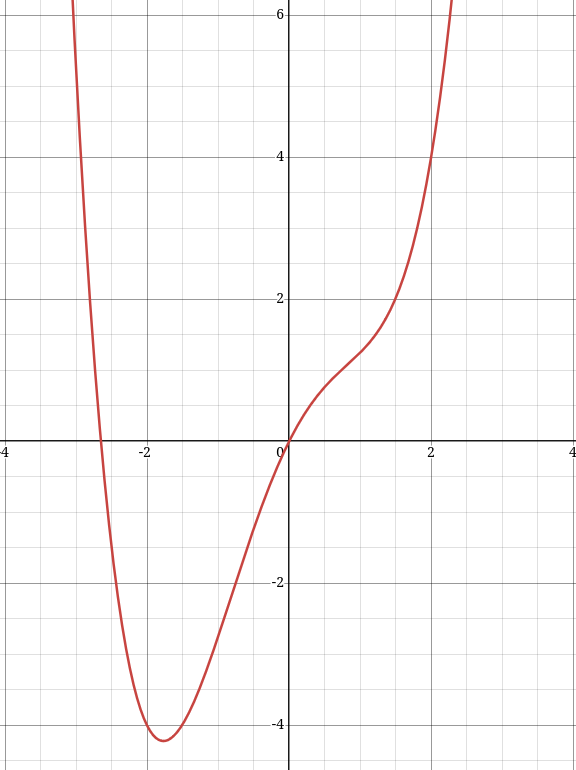
\includegraphics[keepaspectratio]{images/clipboard-3935267595.png}}

}

\caption{Plot of the Objective Function f(x)}

\end{figure}%

I observe that given the code output, the algorithms that did not
converge oscillate between 0 1 0 1, which means that it gets stuck when
the curvature of the graph changes. I think that the graph goes from
concave up to concave down at this point, which will mess up the
gradient descent calculation. The Hessian is the second derivative, or
second order gradient, meaning the concavity of the function will affect
the sign. Given the update step,
\(x_{k+1} = x_k - [\nabla^2f(x_k)]^{-1} \nabla f(x_k)\), we can see that
if the Hessian's sign goes from negative to positive(concave down to
concave up) or vice versa then it will change the sign of the update
step to be gradient ascent(away from the minimum) rather than towards it

\subsubsection{Part (ii) How can you fix the issue reported in
(i)?}\label{part-ii-how-can-you-fix-the-issue-reported-in-i}

I believe that the issue is normally fixed by drawing the graph and
getting and understanding of the shape, and therefore choosing one of
the starting points that does end up converging. However, in cases where
that isn't possible(if the function cannot be plotted or is very
complex), I would try to build a vector of possible starting points and
perform a grid search where we run the algorithm on multiple starting
points and various parameters. This would allow us to find a starting
point where the algorithm would converge. Although the grid search is an
easy fix, switching algorithms is a better fix. From the lecture slides,
there are alternative Newton's algorithms like the Levenberg-Marquard
algorithm, which is a fix for when the Hessian is not positive definite
by essentially translating the Hessian to positive definite through
transforming the eigenvalues of the matrix, which I would implement if
there is too much trouble with the pure Newton's algorithm.

\newpage

\subsection{Problem 2}\label{problem-2}

Consider the data in the train data.csv file. The first 600 columns
correspond to the predictors and the last column to the response y.

\subsubsection{Part (i) Implement that proximal gradient algorithm for
Lasso regression, by modifying appropriately your code from Homework
1.}\label{part-i-implement-that-proximal-gradient-algorithm-for-lasso-regression-by-modifying-appropriately-your-code-from-homework-1.}

Proximal Gradient Descent is good for problems in the form:

\[
\underset{x}{\min} F(x) = f(x) + g(x), \space x \in \mathbb{R}^n
\]

Where f and g are functions with a global minimum, f is differentiable,
and g is not differentiable. In this case, we have
\(MSE=f(x)=\frac{1}{n}||y-X\beta||_2^2\) and \(g(x)=\lambda||\beta||_1\)

\textbf{The Proximal Gradient Descent Algorithm(General):}

\begin{enumerate}
\def\labelenumi{\arabic{enumi}.}
\tightlist
\item
  Select \(x_0 \in \mathbb{R}^n\)
\item
  While stopping criterion \textgreater{} tolerance do:

  \begin{enumerate}
  \def\labelenumii{\arabic{enumii}.}
  \tightlist
  \item
    \(y_k = x_k + \eta_k \nabla{f(x_k)}\)
  \item
    \(x_{k+1} = \text{prox}_{\eta_k,g}(y_k)\)
  \item
    Calculate value of stopping
    criterion(\(|f(x_{k+1}) - f(x_k)| \leq \epsilon\))
  \end{enumerate}
\end{enumerate}

Proximal Operator:
\(\text{prox}_{\eta_k,g}(y_k) = \underset{x}{\text{argmin}}\{ g(x) + \frac{1}{2\eta_k}||x-y_k||^2_2 \}\),
where,

\begin{itemize}
\item
  \(\eta_k\) is the step size at the previous iteration,
\item
  \(y_k\) is the gradient step at the previous iteration,
\item
  \(\text{argmin}\) is the minimum value of the function
\end{itemize}

The Proximal Function for L1-Regularization(LASSO), as shown in class:

\[
\text{prox}_{t,\lambda||\cdot||_1}(z) = S_{t,\lambda}(z) = \text{sign}(z) \cdot \max(|z|-t\lambda,\space0)
\]

\begin{Shaded}
\begin{Highlighting}[]
\CommentTok{\# Params}
\NormalTok{X\_train }\OtherTok{\textless{}{-}}\NormalTok{ train }\SpecialCharTok{\%\textgreater{}\%}
  \FunctionTok{select}\NormalTok{(}\SpecialCharTok{{-}}\NormalTok{y) }\SpecialCharTok{\%\textgreater{}\%}
  \FunctionTok{as.matrix}\NormalTok{()}
\NormalTok{y\_train }\OtherTok{\textless{}{-}}\NormalTok{ train }\SpecialCharTok{\%\textgreater{}\%}
  \FunctionTok{select}\NormalTok{(y) }\SpecialCharTok{\%\textgreater{}\%}
  \FunctionTok{as.matrix}\NormalTok{()}
\NormalTok{X\_val }\OtherTok{\textless{}{-}}\NormalTok{ val }\SpecialCharTok{\%\textgreater{}\%}
  \FunctionTok{select}\NormalTok{(}\SpecialCharTok{{-}}\NormalTok{y) }\SpecialCharTok{\%\textgreater{}\%}
  \FunctionTok{as.matrix}\NormalTok{()}
\NormalTok{y\_val }\OtherTok{\textless{}{-}}\NormalTok{ val }\SpecialCharTok{\%\textgreater{}\%}
  \FunctionTok{select}\NormalTok{(y) }\SpecialCharTok{\%\textgreater{}\%}
  \FunctionTok{as.matrix}\NormalTok{()}


\CommentTok{\# Implement Proximal Gradient Descent}
\NormalTok{proximal\_gradient\_descent\_lasso }\OtherTok{\textless{}{-}} \ControlFlowTok{function}\NormalTok{(X, y, X\_val, y\_val, eta, lambda, tol, max\_iter) \{}
\NormalTok{  n }\OtherTok{\textless{}{-}} \FunctionTok{nrow}\NormalTok{(X)}
\NormalTok{  p }\OtherTok{\textless{}{-}} \FunctionTok{ncol}\NormalTok{(X)}
\NormalTok{  beta }\OtherTok{\textless{}{-}} \FunctionTok{rep}\NormalTok{(}\DecValTok{0}\NormalTok{, p)}
\NormalTok{  obj\_values }\OtherTok{\textless{}{-}} \FunctionTok{numeric}\NormalTok{(max\_iter) }\CommentTok{\# obj values result}
\NormalTok{  eta\_values }\OtherTok{\textless{}{-}} \FunctionTok{numeric}\NormalTok{(max\_iter)  }\CommentTok{\# eta values result}
\NormalTok{  sse\_train\_loss }\OtherTok{\textless{}{-}} \FunctionTok{numeric}\NormalTok{(max\_iter)  }\CommentTok{\# SSE train loss result}
\NormalTok{  sse\_val\_loss }\OtherTok{\textless{}{-}} \FunctionTok{numeric}\NormalTok{(max\_iter)  }\CommentTok{\# SSE test loss result}
\NormalTok{  beta\_values }\OtherTok{\textless{}{-}} \FunctionTok{matrix}\NormalTok{(}\DecValTok{0}\NormalTok{, }\AttributeTok{nrow =}\NormalTok{ max\_iter, }\AttributeTok{ncol =}\NormalTok{ p) }\CommentTok{\# betas result}
  
  
  \CommentTok{\# Objective function: Mean Squared Error (MSE)}
\NormalTok{  obj\_function }\OtherTok{\textless{}{-}} \ControlFlowTok{function}\NormalTok{(beta) \{}
    \FunctionTok{sum}\NormalTok{((X }\SpecialCharTok{\%*\%}\NormalTok{ beta }\SpecialCharTok{{-}}\NormalTok{ y)}\SpecialCharTok{\^{}}\DecValTok{2}\NormalTok{) }\SpecialCharTok{/}\NormalTok{ (}\DecValTok{2} \SpecialCharTok{*}\NormalTok{ n) }\SpecialCharTok{+}\NormalTok{ lambda }\SpecialCharTok{*} \FunctionTok{sum}\NormalTok{(}\FunctionTok{abs}\NormalTok{(beta))}
\NormalTok{  \}}
  
  \CommentTok{\# Gradient function}
\NormalTok{  gradient }\OtherTok{\textless{}{-}} \ControlFlowTok{function}\NormalTok{(beta) \{}
    \FunctionTok{t}\NormalTok{(X) }\SpecialCharTok{\%*\%}\NormalTok{ (X }\SpecialCharTok{\%*\%}\NormalTok{ beta }\SpecialCharTok{{-}}\NormalTok{ y) }\SpecialCharTok{/}\NormalTok{ n}
\NormalTok{  \}}
  
  \CommentTok{\# Proximal Function}
\NormalTok{  prox }\OtherTok{\textless{}{-}} \ControlFlowTok{function}\NormalTok{(eta, lambda, y\_k) \{}
    \FunctionTok{sign}\NormalTok{(y\_k) }\SpecialCharTok{*} \FunctionTok{pmax}\NormalTok{(}\FunctionTok{abs}\NormalTok{(y\_k) }\SpecialCharTok{{-}}\NormalTok{ eta }\SpecialCharTok{*}\NormalTok{ lambda, }\DecValTok{0}\NormalTok{)}
\NormalTok{  \}}
  
  \CommentTok{\# Grad Descent Step}
  \ControlFlowTok{for}\NormalTok{ (iter }\ControlFlowTok{in} \DecValTok{1}\SpecialCharTok{:}\NormalTok{max\_iter) \{}
\NormalTok{    grad }\OtherTok{\textless{}{-}} \FunctionTok{gradient}\NormalTok{(beta)}
    
\NormalTok{    y\_k }\OtherTok{\textless{}{-}}\NormalTok{ beta }\SpecialCharTok{{-}}\NormalTok{ eta }\SpecialCharTok{*}\NormalTok{ grad}
\NormalTok{    beta\_new }\OtherTok{\textless{}{-}} \FunctionTok{prox}\NormalTok{(eta, lambda, y\_k)}
    
    \CommentTok{\# Storing the values for result}
\NormalTok{    eta\_values[iter] }\OtherTok{\textless{}{-}}\NormalTok{ eta}
\NormalTok{    beta\_values[iter, ] }\OtherTok{\textless{}{-}}\NormalTok{ beta\_new}
\NormalTok{    obj\_values[iter] }\OtherTok{\textless{}{-}} \FunctionTok{obj\_function}\NormalTok{(beta\_new)}
    \CommentTok{\# Storing the SSE losses}
    \CommentTok{\# get prediction and calculate SSE{-}train{-}loss}
    \CommentTok{\# y = XB}
\NormalTok{    y\_pred }\OtherTok{\textless{}{-}}\NormalTok{ X }\SpecialCharTok{\%*\%}\NormalTok{ beta\_new}
\NormalTok{    sse\_train\_loss[iter] }\OtherTok{\textless{}{-}} \FunctionTok{sum}\NormalTok{((y }\SpecialCharTok{{-}}\NormalTok{ y\_pred)}\SpecialCharTok{\^{}}\DecValTok{2}\NormalTok{)}
    
    \CommentTok{\# get prediction and calculate SSE{-}val{-}loss}
    \CommentTok{\# y = XB}
\NormalTok{    y\_pred }\OtherTok{\textless{}{-}}\NormalTok{ X\_val }\SpecialCharTok{\%*\%}\NormalTok{ beta\_new}
\NormalTok{    sse\_val\_loss[iter] }\OtherTok{\textless{}{-}} \FunctionTok{sum}\NormalTok{((y\_val }\SpecialCharTok{{-}}\NormalTok{ y\_pred)}\SpecialCharTok{\^{}}\DecValTok{2}\NormalTok{)}
    
    \CommentTok{\# Stop crit}
    \ControlFlowTok{if}\NormalTok{ (}\FunctionTok{norm}\NormalTok{(beta\_new }\SpecialCharTok{{-}}\NormalTok{ beta, }\AttributeTok{type =} \StringTok{"2"}\NormalTok{) }\SpecialCharTok{\textless{}}\NormalTok{ tol) \{}\ControlFlowTok{break}\NormalTok{\}}
    
\NormalTok{    beta }\OtherTok{\textless{}{-}}\NormalTok{ beta\_new}
\NormalTok{  \}}
  
\NormalTok{  beta\_values }\OtherTok{\textless{}{-}}\NormalTok{ beta\_values[}\DecValTok{1}\SpecialCharTok{:}\NormalTok{iter, ]}
\NormalTok{  obj\_values }\OtherTok{\textless{}{-}}\NormalTok{ obj\_values[}\DecValTok{1}\SpecialCharTok{:}\NormalTok{iter]}
\NormalTok{  sse\_train\_loss }\OtherTok{\textless{}{-}}\NormalTok{ sse\_train\_loss[}\DecValTok{1}\SpecialCharTok{:}\NormalTok{iter]}
\NormalTok{  sse\_val\_loss }\OtherTok{\textless{}{-}}\NormalTok{ sse\_val\_loss[}\DecValTok{1}\SpecialCharTok{:}\NormalTok{iter]}

  \FunctionTok{return}\NormalTok{(}\FunctionTok{list}\NormalTok{(}\AttributeTok{iterations=}\NormalTok{iter, }\AttributeTok{beta\_fin=}\NormalTok{beta, }\AttributeTok{beta\_values=}\NormalTok{beta\_values, }\AttributeTok{obj\_values=}\NormalTok{obj\_values, }\AttributeTok{eta\_values=}\NormalTok{eta\_values, }\AttributeTok{eta=}\NormalTok{eta, }\AttributeTok{lambda=}\NormalTok{lambda, }\AttributeTok{sse\_train\_loss=}\NormalTok{sse\_train\_loss, }\AttributeTok{sse\_val\_loss=}\NormalTok{sse\_val\_loss))}
\NormalTok{\}}
\end{Highlighting}
\end{Shaded}

\begin{Shaded}
\begin{Highlighting}[]
\NormalTok{m1 }\OtherTok{\textless{}{-}} \FunctionTok{proximal\_gradient\_descent\_lasso}\NormalTok{(X\_train, y\_train, X\_val, y\_val, }\FloatTok{0.01}\NormalTok{, }\FloatTok{0.1}\NormalTok{, }\FloatTok{1e{-}6}\NormalTok{, }\DecValTok{10000}\NormalTok{)}
\end{Highlighting}
\end{Shaded}

\begin{Shaded}
\begin{Highlighting}[]
\FunctionTok{cat}\NormalTok{(}\StringTok{"Iterations:"}\NormalTok{, m1}\SpecialCharTok{$}\NormalTok{iterations, }\StringTok{"}\SpecialCharTok{\textbackslash{}n}\StringTok{"}\NormalTok{)}
\end{Highlighting}
\end{Shaded}

\begin{verbatim}
Iterations: 6435 
\end{verbatim}

\begin{Shaded}
\begin{Highlighting}[]
\FunctionTok{cat}\NormalTok{(}\StringTok{"Obj Values(Last 10):"}\NormalTok{, }\StringTok{"}\SpecialCharTok{\textbackslash{}n}\StringTok{"}\NormalTok{)}
\end{Highlighting}
\end{Shaded}

\begin{verbatim}
Obj Values(Last 10): 
\end{verbatim}

\begin{Shaded}
\begin{Highlighting}[]
\FunctionTok{tail}\NormalTok{(m1}\SpecialCharTok{$}\NormalTok{obj\_values, }\AttributeTok{n =} \DecValTok{10}\NormalTok{)}
\end{Highlighting}
\end{Shaded}

\begin{verbatim}
 [1] 10.55455 10.55455 10.55455 10.55455 10.55455 10.55455 10.55455 10.55455
 [9] 10.55455 10.55455
\end{verbatim}

\begin{Shaded}
\begin{Highlighting}[]
\FunctionTok{cat}\NormalTok{(}\StringTok{"Final Beta(first 10):"}\NormalTok{, }\StringTok{"}\SpecialCharTok{\textbackslash{}n}\StringTok{"}\NormalTok{)}
\end{Highlighting}
\end{Shaded}

\begin{verbatim}
Final Beta(first 10): 
\end{verbatim}

\begin{Shaded}
\begin{Highlighting}[]
\FunctionTok{print}\NormalTok{(m1}\SpecialCharTok{$}\NormalTok{beta\_fin[}\DecValTok{1}\SpecialCharTok{:}\DecValTok{10}\NormalTok{])}
\end{Highlighting}
\end{Shaded}

\begin{verbatim}
 [1]  0.00000000  0.00000000  0.02960429  0.00000000  0.15895370  0.00000000
 [7]  0.00000000  0.00000000 -0.02223592  0.00000000
\end{verbatim}

\begin{Shaded}
\begin{Highlighting}[]
\FunctionTok{cat}\NormalTok{(}\StringTok{"SSE Train Loss(last 10):"}\NormalTok{, }\StringTok{"}\SpecialCharTok{\textbackslash{}n}\StringTok{"}\NormalTok{)}
\end{Highlighting}
\end{Shaded}

\begin{verbatim}
SSE Train Loss(last 10): 
\end{verbatim}

\begin{Shaded}
\begin{Highlighting}[]
\FunctionTok{tail}\NormalTok{(m1}\SpecialCharTok{$}\NormalTok{sse\_train\_loss, }\AttributeTok{n=}\DecValTok{10}\NormalTok{)}
\end{Highlighting}
\end{Shaded}

\begin{verbatim}
 [1] 5923.782 5923.782 5923.782 5923.782 5923.782 5923.782 5923.782 5923.782
 [9] 5923.782 5923.782
\end{verbatim}

\begin{Shaded}
\begin{Highlighting}[]
\FunctionTok{cat}\NormalTok{(}\StringTok{"SSE Val Loss(last 10):"}\NormalTok{, }\StringTok{"}\SpecialCharTok{\textbackslash{}n}\StringTok{"}\NormalTok{)}
\end{Highlighting}
\end{Shaded}

\begin{verbatim}
SSE Val Loss(last 10): 
\end{verbatim}

\begin{Shaded}
\begin{Highlighting}[]
\FunctionTok{tail}\NormalTok{(m1}\SpecialCharTok{$}\NormalTok{sse\_val\_loss, }\AttributeTok{n=}\DecValTok{10}\NormalTok{)}
\end{Highlighting}
\end{Shaded}

\begin{verbatim}
 [1] 3995.004 3995.003 3995.003 3995.003 3995.003 3995.003 3995.003 3995.003
 [9] 3995.003 3995.003
\end{verbatim}

\subsubsection{\texorpdfstring{Part (ii) To select a good value for the
regularization parameter \(λ\) use the data in the validation data.csv
to calculate the sum-of-squares error validation
loss.}{Part (ii) To select a good value for the regularization parameter λ use the data in the validation data.csv to calculate the sum-of-squares error validation loss.}}\label{part-ii-to-select-a-good-value-for-the-regularization-parameter-ux3bb-use-the-data-in-the-validation-data.csv-to-calculate-the-sum-of-squares-error-validation-loss.}

\begin{Shaded}
\begin{Highlighting}[]
\CommentTok{\# Grid Search Params}
\NormalTok{tol }\OtherTok{\textless{}{-}} \FloatTok{1e{-}6}
\NormalTok{max\_iter }\OtherTok{\textless{}{-}} \DecValTok{10000}
\NormalTok{eta }\OtherTok{\textless{}{-}} \FloatTok{0.01}
\NormalTok{lambdas }\OtherTok{\textless{}{-}} \FunctionTok{c}\NormalTok{(}
  \FloatTok{0.001}\NormalTok{,}
  \FloatTok{0.01}\NormalTok{, }\FloatTok{0.02}\NormalTok{, }\FloatTok{0.05}\NormalTok{, }\FloatTok{0.08}\NormalTok{,}
  \FloatTok{0.1}\NormalTok{, }\FloatTok{0.2}\NormalTok{, }\FloatTok{0.5}\NormalTok{,}
  \DecValTok{1}\NormalTok{, }\DecValTok{2}\NormalTok{, }\DecValTok{5}\NormalTok{, }\DecValTok{10}\NormalTok{, }\DecValTok{20}\NormalTok{, }\DecValTok{50}
\NormalTok{)}
\CommentTok{\#lambdas \textless{}{-} c(0.001, 0.01, 0.1)}

\CommentTok{\# Initialize storing structures}
\NormalTok{models\_df }\OtherTok{\textless{}{-}} \FunctionTok{data.frame}\NormalTok{(}
  \AttributeTok{Model =} \FunctionTok{integer}\NormalTok{(),}
  \AttributeTok{Lambda =} \FunctionTok{numeric}\NormalTok{(),}
  \AttributeTok{Iterations =} \FunctionTok{integer}\NormalTok{(),}
  \AttributeTok{Converged =} \FunctionTok{logical}\NormalTok{(),}
  \AttributeTok{SSE\_Train\_Loss =} \FunctionTok{numeric}\NormalTok{(),}
  \AttributeTok{SSE\_Val\_Loss =} \FunctionTok{numeric}\NormalTok{()}
\NormalTok{)}
\NormalTok{models }\OtherTok{\textless{}{-}} \FunctionTok{list}\NormalTok{()}

\CommentTok{\# Running the Code}
\ControlFlowTok{for}\NormalTok{ (i }\ControlFlowTok{in} \DecValTok{1}\SpecialCharTok{:}\FunctionTok{length}\NormalTok{(lambdas)) \{}
    \CommentTok{\# train the model on specific lambda}
\NormalTok{    lambda }\OtherTok{\textless{}{-}}\NormalTok{ lambdas[i]}
\NormalTok{    result }\OtherTok{\textless{}{-}} \FunctionTok{proximal\_gradient\_descent\_lasso}\NormalTok{(X\_train, y\_train, X\_val, y\_val, eta, lambda, tol, max\_iter)}
    
    \CommentTok{\# get prediction and calculate SSE{-}train{-}loss}
    \CommentTok{\# y = XB}
\NormalTok{    y\_pred }\OtherTok{\textless{}{-}}\NormalTok{ X\_train }\SpecialCharTok{\%*\%}\NormalTok{ result}\SpecialCharTok{$}\NormalTok{beta\_fin}
\NormalTok{    sse\_train\_loss }\OtherTok{\textless{}{-}} \FunctionTok{sum}\NormalTok{((y\_train }\SpecialCharTok{{-}}\NormalTok{ y\_pred)}\SpecialCharTok{\^{}}\DecValTok{2}\NormalTok{)}
    
    \CommentTok{\# get prediction and calculate SSE{-}val{-}loss}
    \CommentTok{\# y = XB}
\NormalTok{    y\_pred }\OtherTok{\textless{}{-}}\NormalTok{ X\_val }\SpecialCharTok{\%*\%}\NormalTok{ result}\SpecialCharTok{$}\NormalTok{beta\_fin}
\NormalTok{    sse\_val\_loss }\OtherTok{\textless{}{-}} \FunctionTok{sum}\NormalTok{((y\_val }\SpecialCharTok{{-}}\NormalTok{ y\_pred)}\SpecialCharTok{\^{}}\DecValTok{2}\NormalTok{)}
    
    \CommentTok{\# Output the model}
    \FunctionTok{cat}\NormalTok{(}\StringTok{"}\SpecialCharTok{\textbackslash{}n}\StringTok{Model:"}\NormalTok{, i, }\StringTok{"| Lambda:"}\NormalTok{, result}\SpecialCharTok{$}\NormalTok{lambda, }\StringTok{"| Iterations:"}\NormalTok{, result}\SpecialCharTok{$}\NormalTok{iterations, }\StringTok{"| Converged?:"}\NormalTok{, result}\SpecialCharTok{$}\NormalTok{iterations }\SpecialCharTok{\textless{}}\NormalTok{ max\_iter, }\StringTok{"| SSE Train Loss:"}\NormalTok{, sse\_train\_loss, }\StringTok{"| SSE Val Loss:"}\NormalTok{, sse\_val\_loss, }\StringTok{"}\SpecialCharTok{\textbackslash{}n}\StringTok{"}\NormalTok{)}
    
    \CommentTok{\# Store row in the results data frame}
\NormalTok{    models\_df }\OtherTok{\textless{}{-}} \FunctionTok{rbind}\NormalTok{(models\_df, }\FunctionTok{data.frame}\NormalTok{(}
      \AttributeTok{Model =}\NormalTok{ i,}
      \AttributeTok{Lambda =}\NormalTok{ result}\SpecialCharTok{$}\NormalTok{lambda,}
      \AttributeTok{Iterations =}\NormalTok{ result}\SpecialCharTok{$}\NormalTok{iterations,}
      \AttributeTok{Converged =}\NormalTok{ result}\SpecialCharTok{$}\NormalTok{iterations }\SpecialCharTok{\textless{}}\NormalTok{ max\_iter,}
      \AttributeTok{SSE\_Train\_Loss =}\NormalTok{ sse\_train\_loss,}
      \AttributeTok{SSE\_Val\_Loss =}\NormalTok{ sse\_val\_loss}
\NormalTok{    ))}
    
    \CommentTok{\# Store the model params in a list for later retrieval}
\NormalTok{    models[[i]] }\OtherTok{\textless{}{-}}\NormalTok{ result}
\NormalTok{\}}
\end{Highlighting}
\end{Shaded}

\begin{verbatim}

Model: 1 | Lambda: 0.001 | Iterations: 10000 | Converged?: FALSE | SSE Train Loss: 523.841 | SSE Val Loss: 18612.82 

Model: 2 | Lambda: 0.01 | Iterations: 10000 | Converged?: FALSE | SSE Train Loss: 1128.191 | SSE Val Loss: 10146.82 

Model: 3 | Lambda: 0.02 | Iterations: 10000 | Converged?: FALSE | SSE Train Loss: 1881.458 | SSE Val Loss: 6926.871 

Model: 4 | Lambda: 0.05 | Iterations: 10000 | Converged?: FALSE | SSE Train Loss: 3670.824 | SSE Val Loss: 4674.736 

Model: 5 | Lambda: 0.08 | Iterations: 7629 | Converged?: TRUE | SSE Train Loss: 5112.683 | SSE Val Loss: 4118.298 

Model: 6 | Lambda: 0.1 | Iterations: 6435 | Converged?: TRUE | SSE Train Loss: 5923.782 | SSE Val Loss: 3995.003 

Model: 7 | Lambda: 0.2 | Iterations: 3440 | Converged?: TRUE | SSE Train Loss: 8755.456 | SSE Val Loss: 4062.508 

Model: 8 | Lambda: 0.5 | Iterations: 2045 | Converged?: TRUE | SSE Train Loss: 15849.07 | SSE Val Loss: 5859.498 

Model: 9 | Lambda: 1 | Iterations: 1099 | Converged?: TRUE | SSE Train Loss: 27946.54 | SSE Val Loss: 10324.96 

Model: 10 | Lambda: 2 | Iterations: 809 | Converged?: TRUE | SSE Train Loss: 39196.53 | SSE Val Loss: 14343.6 

Model: 11 | Lambda: 5 | Iterations: 1 | Converged?: TRUE | SSE Train Loss: 39951.34 | SSE Val Loss: 14548.27 

Model: 12 | Lambda: 10 | Iterations: 1 | Converged?: TRUE | SSE Train Loss: 39951.34 | SSE Val Loss: 14548.27 

Model: 13 | Lambda: 20 | Iterations: 1 | Converged?: TRUE | SSE Train Loss: 39951.34 | SSE Val Loss: 14548.27 

Model: 14 | Lambda: 50 | Iterations: 1 | Converged?: TRUE | SSE Train Loss: 39951.34 | SSE Val Loss: 14548.27 
\end{verbatim}

\begin{Shaded}
\begin{Highlighting}[]
\NormalTok{models\_df}
\end{Highlighting}
\end{Shaded}

Model Lambda Iterations Converged SSE\_Train\_Loss SSE\_Val\_Loss 1 1
1e-03 10000 FALSE 523.841 18612.824 2 2 1e-02 10000 FALSE 1128.191
10146.815 3 3 2e-02 10000 FALSE 1881.458 6926.871 4 4 5e-02 10000 FALSE
3670.824 4674.736 5 5 8e-02 7629 TRUE 5112.683 4118.298 6 6 1e-01 6435
TRUE 5923.782 3995.003 7 7 2e-01 3440 TRUE 8755.456 4062.508 8 8 5e-01
2045 TRUE 15849.066 5859.498 9 9 1e+00 1099 TRUE 27946.536 10324.959 10
10 2e+00 809 TRUE 39196.533 14343.601 11 11 5e+00 1 TRUE 39951.338
14548.269 12 12 1e+01 1 TRUE 39951.338 14548.269 13 13 2e+01 1 TRUE
39951.338 14548.269 14 14 5e+01 1 TRUE 39951.338 14548.269

\begin{Shaded}
\begin{Highlighting}[]
\NormalTok{latex\_table }\OtherTok{\textless{}{-}} \FunctionTok{xtable}\NormalTok{(models\_df, }\AttributeTok{digits =} \DecValTok{4}\NormalTok{, }\AttributeTok{caption =} \StringTok{"Model Results For Different Lambdas"}\NormalTok{)}
\FunctionTok{print}\NormalTok{(latex\_table, }\AttributeTok{include.rownames =} \ConstantTok{FALSE}\NormalTok{)}
\end{Highlighting}
\end{Shaded}

\% latex table generated in R 4.5.0 by xtable 1.8-4 package \% Wed Jun 4
21:48:25 2025

\begin{table}[ht]
\centering
\begin{tabular}{rrrlrr}
  \hline
Model & Lambda & Iterations & Converged & SSE\_Train\_Loss & SSE\_Val\_Loss \\ 
  \hline
    1 & 0.0010 & 10000 & FALSE & 523.8410 & 18612.8235 \\ 
      2 & 0.0100 & 10000 & FALSE & 1128.1908 & 10146.8151 \\ 
      3 & 0.0200 & 10000 & FALSE & 1881.4576 & 6926.8709 \\ 
      4 & 0.0500 & 10000 & FALSE & 3670.8241 & 4674.7357 \\ 
      5 & 0.0800 &  7629 & TRUE & 5112.6825 & 4118.2976 \\ 
      6 & 0.1000 &  6435 & TRUE & 5923.7823 & 3995.0029 \\ 
      7 & 0.2000 &  3440 & TRUE & 8755.4563 & 4062.5080 \\ 
      8 & 0.5000 &  2045 & TRUE & 15849.0656 & 5859.4978 \\ 
      9 & 1.0000 &  1099 & TRUE & 27946.5359 & 10324.9595 \\ 
     10 & 2.0000 &   809 & TRUE & 39196.5329 & 14343.6008 \\ 
     11 & 5.0000 &     1 & TRUE & 39951.3385 & 14548.2692 \\ 
     12 & 10.0000 &     1 & TRUE & 39951.3385 & 14548.2692 \\ 
     13 & 20.0000 &     1 & TRUE & 39951.3385 & 14548.2692 \\ 
     14 & 50.0000 &     1 & TRUE & 39951.3385 & 14548.2692 \\ 
   \hline
\end{tabular}
\caption{Model Results For Different Lambdas} 
\end{table}

\subsubsection{Part(iii) Show a plot of the training and validation loss
as a function of
iterations.}\label{partiii-show-a-plot-of-the-training-and-validation-loss-as-a-function-of-iterations.}

Getting the Data:

\begin{Shaded}
\begin{Highlighting}[]
\CommentTok{\# build a big data frame}
\NormalTok{big\_df }\OtherTok{\textless{}{-}} \FunctionTok{data.frame}\NormalTok{(}
  \AttributeTok{Lambda =} \FunctionTok{numeric}\NormalTok{(),}
  \AttributeTok{Iterations =} \FunctionTok{integer}\NormalTok{(),}
  \AttributeTok{SSE\_Train\_Loss =} \FunctionTok{numeric}\NormalTok{(),}
  \AttributeTok{SSE\_Val\_Loss =} \FunctionTok{numeric}\NormalTok{()}
\NormalTok{)}
\CommentTok{\# get the SSE data and put it in the data frame}
\ControlFlowTok{for}\NormalTok{(model }\ControlFlowTok{in}\NormalTok{ models) \{}
\NormalTok{  sub\_df }\OtherTok{\textless{}{-}} \FunctionTok{cbind}\NormalTok{(}\AttributeTok{Lambda =}\NormalTok{ model}\SpecialCharTok{$}\NormalTok{lambda, }\AttributeTok{Iteration =} \DecValTok{1}\SpecialCharTok{:}\NormalTok{model}\SpecialCharTok{$}\NormalTok{iterations, }\AttributeTok{SSE\_Train\_Loss =}\NormalTok{ model}\SpecialCharTok{$}\NormalTok{sse\_train\_loss, }\AttributeTok{SSE\_Val\_Loss =}\NormalTok{ model}\SpecialCharTok{$}\NormalTok{sse\_val\_loss)}
\NormalTok{  big\_df }\OtherTok{\textless{}{-}} \FunctionTok{rbind}\NormalTok{(big\_df, sub\_df)}
\NormalTok{\}}

\NormalTok{big\_df }\OtherTok{\textless{}{-}}\NormalTok{ big\_df }\SpecialCharTok{\%\textgreater{}\%}
  \FunctionTok{mutate}\NormalTok{(}\AttributeTok{Lambda =} \FunctionTok{factor}\NormalTok{(Lambda))}

\FunctionTok{head}\NormalTok{(big\_df)}
\end{Highlighting}
\end{Shaded}

\begin{verbatim}
  Lambda Iteration SSE_Train_Loss SSE_Val_Loss
1  0.001         1       38360.91     14184.63
2  0.001         2       36873.68     13842.38
3  0.001         3       35481.71     13519.99
4  0.001         4       34177.75     13216.04
5  0.001         5       32955.15     12929.25
6  0.001         6       31807.80     12658.40
\end{verbatim}

Plotting Training Loss:

\begin{Shaded}
\begin{Highlighting}[]
\NormalTok{big\_df }\SpecialCharTok{\%\textgreater{}\%}
  \FunctionTok{ggplot}\NormalTok{(}\FunctionTok{aes}\NormalTok{(}\AttributeTok{x=}\NormalTok{Iteration, }\AttributeTok{y=}\NormalTok{SSE\_Train\_Loss, }\AttributeTok{color=}\NormalTok{Lambda)) }\SpecialCharTok{+} 
    \FunctionTok{geom\_line}\NormalTok{() }\SpecialCharTok{+} 
    \FunctionTok{theme\_minimal}\NormalTok{() }\SpecialCharTok{+} 
    \FunctionTok{ggtitle}\NormalTok{(}\StringTok{"Training Loss"}\NormalTok{) }\SpecialCharTok{+} 
    \FunctionTok{ylab}\NormalTok{(}\StringTok{"SSE Train Loss"}\NormalTok{)}
\end{Highlighting}
\end{Shaded}

\pandocbounded{\includegraphics[keepaspectratio]{506021334_stats102b_hw4_files/figure-pdf/2-3-train-loss-1.pdf}}

Plotting Validation Loss:

\begin{Shaded}
\begin{Highlighting}[]
\NormalTok{big\_df }\SpecialCharTok{\%\textgreater{}\%}
  \FunctionTok{ggplot}\NormalTok{(}\FunctionTok{aes}\NormalTok{(}\AttributeTok{x=}\NormalTok{Iteration, }\AttributeTok{y=}\NormalTok{SSE\_Val\_Loss, }\AttributeTok{color=}\NormalTok{Lambda)) }\SpecialCharTok{+} 
    \FunctionTok{geom\_line}\NormalTok{() }\SpecialCharTok{+} 
    \FunctionTok{theme\_minimal}\NormalTok{() }\SpecialCharTok{+} 
    \FunctionTok{ggtitle}\NormalTok{(}\StringTok{"Validation Loss"}\NormalTok{) }\SpecialCharTok{+} 
    \FunctionTok{ylab}\NormalTok{(}\StringTok{"SSE Validation Loss"}\NormalTok{)}
\end{Highlighting}
\end{Shaded}

\pandocbounded{\includegraphics[keepaspectratio]{506021334_stats102b_hw4_files/figure-pdf/2-3-validation-loss-1.pdf}}

\subsubsection{\texorpdfstring{Part(iv) Report the number of regression
coefficients estimated as zero based on the best value of \(λ\) you
selected.}{Part(iv) Report the number of regression coefficients estimated as zero based on the best value of λ you selected.}}\label{partiv-report-the-number-of-regression-coefficients-estimated-as-zero-based-on-the-best-value-of-ux3bb-you-selected.}

Output the table of the best model

\begin{Shaded}
\begin{Highlighting}[]
\NormalTok{models\_df }\SpecialCharTok{\%\textgreater{}\%}
  \FunctionTok{arrange}\NormalTok{(SSE\_Val\_Loss)}
\end{Highlighting}
\end{Shaded}

\begin{verbatim}
   Model Lambda Iterations Converged SSE_Train_Loss SSE_Val_Loss
1      6  1e-01       6435      TRUE       5923.782     3995.003
2      7  2e-01       3440      TRUE       8755.456     4062.508
3      5  8e-02       7629      TRUE       5112.683     4118.298
4      4  5e-02      10000     FALSE       3670.824     4674.736
5      8  5e-01       2045      TRUE      15849.066     5859.498
6      3  2e-02      10000     FALSE       1881.458     6926.871
7      2  1e-02      10000     FALSE       1128.191    10146.815
8      9  1e+00       1099      TRUE      27946.536    10324.959
9     10  2e+00        809      TRUE      39196.533    14343.601
10    11  5e+00          1      TRUE      39951.338    14548.269
11    12  1e+01          1      TRUE      39951.338    14548.269
12    13  2e+01          1      TRUE      39951.338    14548.269
13    14  5e+01          1      TRUE      39951.338    14548.269
14     1  1e-03      10000     FALSE        523.841    18612.824
\end{verbatim}

The best lambda that we found was 0.1

\begin{Shaded}
\begin{Highlighting}[]
\CommentTok{\# print(models[[6]]$beta\_fin)}
\NormalTok{models[[}\DecValTok{6}\NormalTok{]]}\SpecialCharTok{$}\NormalTok{lambda}
\end{Highlighting}
\end{Shaded}

\begin{verbatim}
[1] 0.1
\end{verbatim}

\begin{Shaded}
\begin{Highlighting}[]
\FunctionTok{sum}\NormalTok{(}\FunctionTok{abs}\NormalTok{(models[[}\DecValTok{6}\NormalTok{]]}\SpecialCharTok{$}\NormalTok{beta\_fin) }\SpecialCharTok{\textless{}} \FloatTok{1e{-}6}\NormalTok{)}
\end{Highlighting}
\end{Shaded}

\begin{verbatim}
[1] 380
\end{verbatim}

There were 380 coefficients that were shrunk to 0 for the model that had
a lambda of 0.1




\end{document}
